\documentclass[tikz,border=8pt]{standalone}
\usepackage{amsmath}
\usepackage{amssymb}
\usetikzlibrary{arrows.meta,calc,positioning}

\definecolor{basisblue}{HTML}{2F6F9F}
\definecolor{basisgreen}{HTML}{5F7F55}
\definecolor{basisgold}{HTML}{A66F00}
\definecolor{textgray}{HTML}{2F3437}
\definecolor{linegray}{HTML}{AEB7BC}
\definecolor{softgray}{HTML}{F5F7F8}

\begin{document}
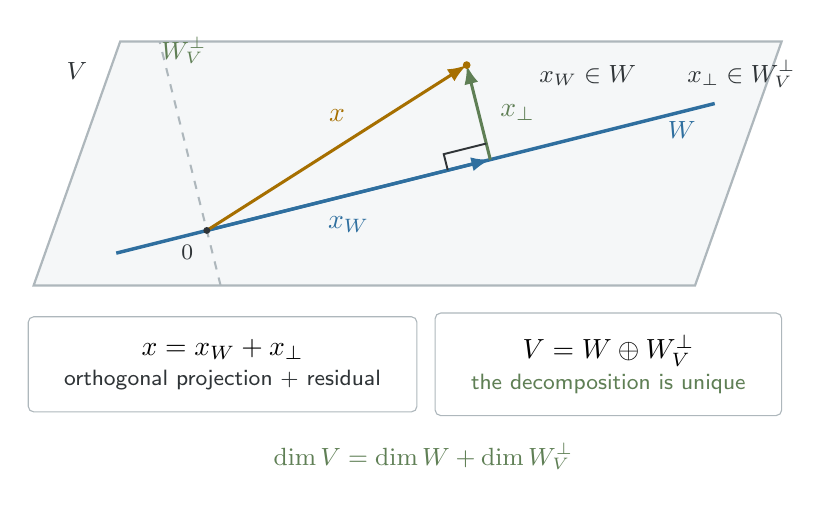
\begin{tikzpicture}[
  font=\sffamily,
  >=Latex,
  vector/.style={-{Latex[length=2.4mm]}, line width=1.1pt},
  guide/.style={draw=linegray, dashed, line width=0.75pt},
  label/.style={font=\sffamily\bfseries\small, text=textgray},
  smallnote/.style={font=\sffamily\small, text=textgray, align=center},
  mathnote/.style={font=\sffamily\footnotesize, text=textgray, align=center},
  stage/.style={
    draw=linegray,
    fill=white,
    rounded corners=2pt,
    inner xsep=13pt,
    inner ysep=8pt,
    align=center
  }
]

% Ambient vector space V, drawn schematically as a plane.
\fill[softgray] (-4.75,-1.55) -- (3.65,-1.55) -- (4.75,1.55) -- (-3.65,1.55) -- cycle;
\draw[draw=linegray, line width=0.8pt]
  (-4.75,-1.55) -- (3.65,-1.55) -- (4.75,1.55) -- (-3.65,1.55) -- cycle;
\node[label] at (-4.20,1.18) {$V$};

\coordinate (O) at (-2.55,-0.85);
\coordinate (P) at (1.05,0.05);
\coordinate (X) at (0.75,1.25);

% The subspace W and its orthogonal complement through the origin.
\draw[draw=basisblue, line width=1.25pt]
  ($(O)+(-1.15,-0.2875)$) -- ($(O)+(6.45,1.6125)$);
\node[smallnote, text=basisblue, anchor=west] at (3.18,0.43) {$W$};

\draw[guide]
  (-2.375,-1.55) -- (-3.15,1.55);
\node[smallnote, text=basisgreen, anchor=south west] at (-3.25,1.14) {$W_V^{\perp}$};

% Orthogonal decomposition x = x_W + x_perp.
\draw[vector, draw=basisblue] (O) -- (P)
  node[midway, below=4pt, text=basisblue] {$x_W$};
\draw[vector, draw=basisgreen] (P) -- (X)
  node[midway, right=4pt, text=basisgreen] {$x_{\perp}$};
\draw[vector, draw=basisgold] (O) -- (X)
  node[pos=0.58, above left=1pt, text=basisgold] {$x$};

\fill[textgray] (O) circle (1.25pt);
\node[mathnote, anchor=north east] at ($(O)+(-0.05,-0.06)$) {$0$};
\fill[basisgold] (X) circle (1.4pt);

% Right-angle marker at the projection x_W.
\coordinate (A) at ($(P)!0.15!(O)$);
\coordinate (B) at ($(P)!0.17!(X)$);
\draw[draw=textgray, line width=0.7pt]
  (A) -- ($(A)+(B)-(P)$) -- (B);

\node[smallnote, anchor=west] at (1.55,1.14)
  {$x_W\in W$\qquad $x_{\perp}\in W_V^{\perp}$};

% Summary statements.
\node[stage, minimum width=4.25cm] at (-2.35,-2.55)
  {$x=x_W+x_{\perp}$\\[-1pt]
   \textcolor{textgray}{\footnotesize orthogonal projection + residual}};

\node[stage, minimum width=4.25cm] at (2.55,-2.55)
  {$V=W\oplus W_V^{\perp}$\\[-1pt]
   \textcolor{basisgreen}{\footnotesize the decomposition is unique}};

\node[smallnote, text=basisgreen] at (0.20,-3.72)
  {$\dim V=\dim W+\dim W_V^{\perp}$};

\end{tikzpicture}
\end{document}
